\documentclass[12pt]{article}
\usepackage[top=1in, bottom=1in, left=.75in, right=.75in]{geometry}
\usepackage{amsmath, enumerate}
\usepackage{fancyhdr}
\usepackage{graphicx, xcolor, setspace, array, adjustbox}
\usepackage{txfonts}
\usepackage{multicol,coordsys,pgfplots}
\usepackage[scaled=0.86]{helvet}
\renewcommand{\emph}[1]{\textsf{\textbf{#1}}}
\usepackage{anyfontsize}
% \usepackage{times}
% \usepackage[lf]{MinionPro}
%\usepackage{tikz,pgfplots}

\usepackage{tikz}
\usetikzlibrary{calc,trees,positioning,arrows,fit,shapes,through, backgrounds}
\usetikzlibrary{patterns}

\usetikzlibrary{decorations.markings}
\usetikzlibrary{arrows}

%\def\degC{{}^\circ{\rm C}}
\def\ra{\rightarrow}
\usetikzlibrary{calc,arrows.meta}
\pgfplotsset{compat = newest}
\newcommand{\blank}[1]{\rule{#1}{0.75pt}}

\pgfplotsset{my style/.append style={axis x line=middle, axis y line=
middle, xlabel={$x$}, ylabel={$y$}}}

%axis equal

%yticklabels={,,} , xticklabels={,,}

% \setmainfont{Times}
% \def\sansfont{Lucida Grande Bold}
\parindent 0pt
\parskip 4pt
\pagestyle{fancy}
\fancyfoot[C]{\emph{\thepage}}
\fancyfoot[R]{} %%%%%% <-- Version Info
\fancyhead[L]{\ifnum \value{page} > 1\relax\emph{Math F113X: Exam 2}\fi}
\fancyhead[R]{\ifnum \value{page} > 1\relax\emph{Fall 2025}\fi}
\headheight 15pt
\renewcommand{\headrulewidth}{0pt}
\renewcommand{\footrulewidth}{0pt}
\let\ds\displaystyle
\def\continued{{\emph {Continued....}}}
\def\continuing{{\emph {Problem \arabic{probcount} continued....}}\par\vskip 4pt}


\newcounter{probcount}
\newcounter{subprobcount}
\newcommand{\thesubproblem}{\emph{\alph{subprobcount}.}}
\def\problem#1{\setcounter{subprobcount}{0}%
\addtocounter{probcount}{1}{\emph{\arabic{probcount}.\hskip 1em(#1)}}\par}
\def\subproblem#1{\par\hangindent=1em\hangafter=0{%
\addtocounter{subprobcount}{1}\thesubproblem\emph{#1}\hskip 1em}}
\def\probskip{\vskip 10pt}
\def\medprobskip{\vskip 2in}
\def\subprobskip{\vskip 45pt}
\def\bigprobskip{\vskip 4in}


\newenvironment{subproblems}{%
\begin{enumerate}%
\setcounter{enumi}{\value{subprobcount}}%
\renewcommand{\theenumi}{\emph{\alph{enumi}}}}%
{\setcounter{subprobcount}{\value{enumi}}\end{enumerate}}


\newcommand{\be}{\begin{enumerate}}
\newcommand{\ee}{\end{enumerate}}


\newcommand{\ans}[1][1in]{\rule{#1}{.5pt}}



\begin{document}

{\emph{\fontsize{26}{28}\selectfont Fall 2025 \hfill
%{\fontsize{32}{36}\selectfont Calculus 1: Midterm 1}
\hfill Math F113X}}

\begin{center}
{\emph{%\fontsize{26}{28}\selectfont Spring 2024 
%%\hfill
{\fontsize{32}{36}\selectfont Exam 2}
%%\hfill Math F251X}
}}
\end{center}

%\vskip 2cm
\strut\vtop{\halign{\emph#\hskip 0.5em\hfil&#\hbox to 2in{\hrulefill}\cr
\emph{\fontsize{18}{22}\selectfont Name:}&\cr
%\noalign{\vskip 10pt}
%\emph{\fontsize{18}{22}\selectfont Student Id:}&\cr
%\noalign{\vskip 10pt}
%\emph{\fontsize{18}{22}\selectfont Calculator Model:}&\cr
}}
\hfill
\vtop{\halign{\emph{\fontsize{18}{22}\selectfont #}\hfil& \emph{\fontsize{18}{22}\selectfont\hskip 0.5ex $\square$ #}\hfil\cr
Section: & 10:30 am (Leah Berman )\cr
\noalign{\vskip 4pt}
         & 11:45 am (Kevin Meek)\cr
         \noalign{\vskip 4pt}
         & online (Kevin Meek)\cr
}}

\vfill
{\fontsize{18}{22}\selectfont\emph{Rules:}}

\begin{itemize}
\item Partial credit will be awarded, but you must show your work.

\item You may have 1/2 of a standard page of paper ($8.5''\times 5.5''$)  of notes, both sides.

\item Calculators are allowed. 

\item Place a box around your  \fbox{FINAL ANSWER} to each question where appropriate.

\item Turn off anything that might go beep during the exam.

\end{itemize}

%If you need extra space, you can use the back sides of the pages.
%Please make it obvious  when you have done so.



Good luck!

\vfill
\def\emptybox{\hbox to 2em{\vrule height 16pt depth 8pt width 0pt\hfil}}
\def\tline{\noalign{\hrule}}
\centerline{\vbox{\offinterlineskip
{
\bf\sf\fontsize{18pt}{22pt}\selectfont
\hrule
\halign{
\vrule#&\strut\quad\hfil#\hfil\quad&\vrule#&\quad\hfil#\hfil\quad
&\vrule#&\quad\hfil#\hfil\quad&\vrule#\cr
height 3pt&\omit&&\omit&&\omit&\cr
&Problem&&Possible&&Score&\cr\tline
height 3pt&\omit&&\omit&&\omit&\cr
&1&& 10	&&\emptybox&\cr\tline
&2&& 10	&&\emptybox&\cr\tline
&3&& 12	&&\emptybox&\cr\tline
&4&& 16	&&\emptybox&\cr\tline
&5&& 14	&&\emptybox&\cr\tline
&6&& 10	&&\emptybox&\cr\tline
&7&& 16	&&\emptybox&\cr\tline
&8&& 12	&&\emptybox&\cr\tline
%&9&& 8	&&\emptybox&\cr\tline \tline
&Extra Credit&&(6)&&\emptybox&\cr\tline
&Total&&100&&\emptybox&\cr
}\hrule}}}

\newpage
%Page 1%

%%%%%%%%%%%
%warm up definitions
%%%%
\problem{10 points} On October 21, the cheapest available one-way, non-stop flights on Alaska Airlines between selected cities for flights on November 15, 2025, are listed in the following table. A $-$ in the table means there is no available non-stop flight.

\begin{tabular}{ c|| c| c | c | c | c}
& Anchorage (ANC) & Seattle (SEA) & Honolulu (HNL) & Los Angeles (LAX)\\ \hline \hline
Fairbanks (FAI) &   \$109 & \$179 & $-$ & $-$ \\ \hline
Anchorage (ANC)  &&  \$188 & \$208 & \$169 \\ \hline
Seattle (SEA)  & &  & \$169 & \$229 \\\hline
Honolulu (HNL) &&&& \$229
\end{tabular}  

 Construct a weighted graph that represents the data. Make sure that your vertices are labeled in a useful way and that the edges and weights are clear.

\vfill

%Give real world examples
%%%%
 \problem{10 points} Describe a \emph{graph} that models a real world situation in which you would want to find each of the following. Explain what the \emph{vertices}, \emph{edges}, and \emph{weights} represent, and what the circuit would tell you.
 
 	\begin{subproblems}
	\item a minimum weight Hamiltonian circuit.
	
	\vfill
	
	\item an Euler circuit.	
	
\vfill

	\end{subproblems}



\newpage
% Page 2 %

%%%
%Kruskals

\newcommand{\pic}{
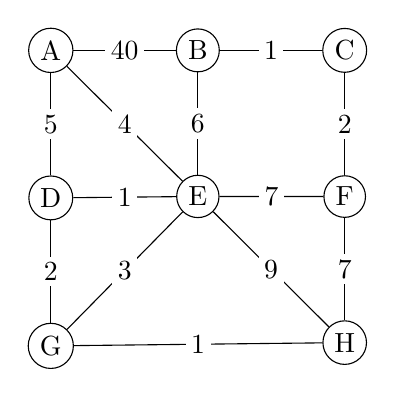
\begin{tikzpicture}
\pgfmathsetmacro{\rr}{1.3}
\tikzstyle{vtx}=[draw, circle, inner sep = 2 pt, node distance=2cm]
\tikzstyle{lbl}=[midway, inner sep = 2 pt, fill = white]

\node[vtx] (A)  {A};
\node[vtx, right  =  \rr of A] (B) {B};
\node[vtx, right  =   \rr of B] (C) {C};
\node[vtx, below =  \rr of A] (D) {D};
\node[vtx, below =  \rr of B] (E) {E};
\node[vtx, below =  \rr of C] (F) {F};
\node[vtx, below =  \rr of D] (G) {G};
\node[vtx, below =  \rr of F] (H) {H};
\foreach \i/\j/\k in {A/B/40, B/C/1, C/F/2, A/D/5, B/E/6, D/E/1, E/F/7, E/G/3, E/H/9, G/H/1, D/G/2, F/H/7, A/E/4  }{\draw (\i) -- node[lbl]{\k} (\j);}
\end{tikzpicture}
}

\newcommand{\blankpic}{
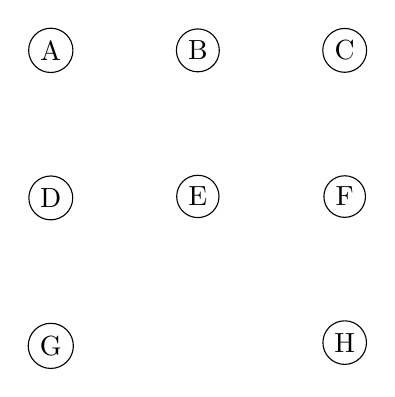
\begin{tikzpicture}
\tikzstyle{vtx}=[draw, circle, inner sep = 2 pt, node distance=2cm]
\tikzstyle{lbl}=[midway, inner sep = 2 pt, fill = white]
\pgfmathsetmacro{\rr}{1.3}

\node[vtx] (A)  {A};
\node[vtx, right  =  \rr of A] (B) {B};
\node[vtx, right  =   \rr of B] (C) {C};
\node[vtx, below =  \rr of A] (D) {D};
\node[vtx, below =  \rr of B] (E) {E};
\node[vtx, below =  \rr of C] (F) {F};
\node[vtx, below =  \rr of D] (G) {G};
\node[vtx, below =  \rr of F] (H) {H};
%\foreach \i/\j/\k in {A/B/15, B/C/1, C/F/2, A/D/5, B/E/10, D/E/1, E/F/7, E/G/3, E/H/9, G/H/1, D/G/2, F/H/7  }{\draw (\i) -- node[lbl]{\k} (\j);}
\end{tikzpicture}

}

\newcommand{\sorted}{
\begin{adjustbox}{valign=t,minipage={.4\textwidth}}
\begin{tabular}{ c | c | p{.8in}}
Sorted edges & weight & used? \\ \hline
$BC$ & 1 &\\ \hline
$DE$ & 1 &\\ \hline
$GH$ &1& \\ \hline
$CF$ & 2 &\\ \hline
$DG$ & 2&\\ \hline
$EG$ & 3&\\ \hline
$AE$ & 4 &\\ \hline
\end{tabular}
\end{adjustbox}
\hspace{1cm}
\begin{adjustbox}{valign=t,minipage={.4\textwidth}}
\begin{tabular}{ c | c | p{.8in}}
Sorted edges & weight & used? \\ \hline
$AD$ & 5&\\ \hline
$BE$ & 6 & \\ \hline
$EF$ & 7 & \\ \hline
$FH$ & 7 &\\ \hline
$EH$ & 9&\\ \hline
$AB$ & 40 &\\  \hline
 \end{tabular}
 \end{adjustbox}

}


%%%
\problem{12 points} 
Recall that Kruskal's Algorithm says the following:

\bigskip

\fbox{Kruskal's Algorithm:} Select the cheapest edge in the graph that does not create a circuit. Stop when a spanning tree is obtained. Break  ties by choosing the edge that comes earlier in the alphabet.

\begin{subproblems}
\item Use Kruskal's Algorithm to determine a \emph{minimum cost spanning tree} in the following graph. 

\begin{itemize}

\item Construct a minimum cost spanning tree in the second graph, with the \emph{edges labeled with their weights}.

\item Keep track of the steps of the algorithm, the edges that you are using, and the weights, in the table below.
\end{itemize}

For convenience, the edges of the graph are listed in sorted order by weight in the table below.

\vspace{1cm}


\begin{adjustbox}{valign=t,minipage={.4\textwidth}}

\pic

\end{adjustbox}
%%%
\hfill
%%%%%%%%
\begin{adjustbox}{valign=t,minipage={.4\textwidth}}

\blankpic

\end{adjustbox}

%\vspace{1cm}

\vspace{1cm}



\sorted


 
\vspace{1cm}

 
\item What is the total cost of the spanning tree you found? \ans
 
\end{subproblems}

\newpage
% page 3 %

%%%
%Cheapest link
%%%
\problem{16 points} 
\fbox{Sorted Edges / Cheapest Link Algorithm:}  Select the cheapest edge in the graph that does not create a vertex of degree 3 or close the circuit too soon. Break any ties by choosing the edge that comes earlier in the alphabet. 

\begin{subproblems}
\item Use \emph{Sorted Edges / Cheapest Link Algorithm} to find a \emph{Hamiltonian circuit} in the following graph. 



Keep track of the cycle, along with the weights, in the second graph.

For convenience, the edges of the graph, sorted by weight, are listed in order in the table below.

\bigskip

\vspace{1cm}

\begin{adjustbox}{valign=t,minipage={.4\textwidth}}

\pic

\end{adjustbox}
%%%
\hfill
%%%%%%%%
\begin{adjustbox}{valign=t,minipage={.4\textwidth}}


\blankpic

\end{adjustbox}

\vspace{1cm}


\sorted
\vspace{1cm}


 
\item Write the Hamiltonian circuit you found, beginning with vertex $A$. 

\hrulefill


\item What is the total weight of the Hamiltonian circuit? \ans

\item Is this the cheapest possible Hamiltonian circuit in this graph? \ans \  Explain your answer below.
\vfill
 
\end{subproblems}

\newpage
%page 5%

\newcommand{\eulerpic}[1]{
\begin{tikzpicture}[baseline=(current bounding box.center),lbl/.style={inner sep = 1pt, fill = white}, scale = #1]
\tikzstyle{vtx}=[circle, draw, inner sep=1pt]
\node at (-1,0){};
\node[vtx] (a) at (0,2) {A};
\node[vtx] (b) at (0,1) {B};
\node[vtx] (c) at (0,0){C};
\node[vtx] (d) at (0,-1){D};
\node[vtx] (e) at (1,1){E};
\node[vtx] (f) at (1,0){F};
\node[vtx] (g) at (1,2){G};
\node[vtx] (h) at (2,1){H};
\node[vtx] (i) at (2,0){I};
\foreach \i/\j in {a/b,b/c,c/d,f/e,e/g,g/h,h/i,i/f,b/e,c/f,e/h, a/g}{\draw (\i) -- (\j);}
\end{tikzpicture}

}

\problem{14 points} 
\begin{subproblems}
%\begin{minipage}{12cm}
%	\emph{a.}  

\item Explain why the graph to the right does not contain an Euler circuit.

\hfill
\eulerpic{1}	
	
	
%	\emph{b.} 
\item Eulerize the graph on the copy of the graph below \emph{using as few edge duplications as possible.} Make your added edges very clear!	


%\end{minipage}


%\hfill 

\begin{center}

\eulerpic{1.5}

\end{center}

Added edges: \hrulefill

\vspace{.5cm}

%\vfill

%\begin{minipage}{12cm}
%\emph{c.} 

\item Find an \emph{Euler circuit} in the eulerized graph by \emph{drawing} the circuit on the  graph \emph{below this problem} and \emph{listing} the vertices of the circuit in the blank below. (You will have to add your edges from part \emph{b} in again!)

Offset your circuit slightly from the graph so that it is clear where the circuit is.

\vspace{.1in}


%\end{minipage}
%\hfill
\begin{center}

\eulerpic{1.5}

\end{center}

\vspace{1cm}

Euler circuit:  \hrulefill

\end{subproblems}

\newpage


%%%
%%%%%%%%%% scheduling digraph - Kevin %%%%%%%%%%%%




\problem{10 points} Construct a \emph{scheduling digraph} corresponding to the following list of tasks and dependencies.

\begin{tabular}{c | c | c}
Task & Time & dependency\\
\hline
A & 1 hours & \\
B & 4 hours & \\
C & 6 hour & \\
D & 7 hours & A\\
E & 2 hour & A,B \\
F & 3 hours & D, E\\
G & 5 hour & C,D,E \\
\end{tabular}
\vfill



% page 6 %



%%%
% priority lists, backflow
%%%



\def\r{1}
\def\s{.9}
\newcommand{\anotherdigraph}{\begin{tikzpicture}[vtx/.style={draw, circle, inner sep = 3pt, %font = \scriptsize
}, myto/.style={-latex, shorten >=2pt, shorten <=2pt
}, node distance = \r cm]

\node[vtx, label=above:{$A(3)$}, ] (A) at (0,0){};
\node[vtx, right = 2*\r of A, label=above:{ $B(5)$}] (B) {};
\node[vtx, below = of A, label=above:{ $C(7)$}] (C) {};
\node[vtx, right = 2*\r of C, label=above:{ $D(4)$}] (D) {};
\node[vtx, right = 2*\r of D, label=above:{ $E(1)$}] (E) {};
\node[vtx, below = of C, label=above:{ $F(2)$}] (F) {};
\foreach \i/\j in {A/B,C/D,D/E,B/E,F/D}{\draw[myto] (\i) -- (\j);}
% \draw[myto] (A) to[bend left = 20] (D);
\end{tikzpicture}
}

\bigskip


%%%%%%%%%%%%%%% scheduling - Kevin %%%%%%%%%%%%%
\problem{14 points} 



% \newcommand{\anotherdigraph}{\begin{tikzpicture}[vtx/.style={draw, circle, inner sep = 3pt, %font = \scriptsize
% }, myto/.style={-latex, shorten >=2pt, shorten <=2pt
% }, node distance = \r cm]
% \node[vtx, label=above:{$A(10)$}, ] (A) at (0,0){};
% \node[vtx, below = \s cm of A, label=above:{ $B(5)$}] (B) {};
% \node[vtx, below =\s cm of B, label=above:{ $F(3)$}] (F) {};
% \node[vtx, right = of B, label=above:{ $C(4)$}] (C) {};
% \node[vtx, right = 2*\r of C, label=right:{ $D(1)$}] (D) {};
% \node[vtx, below =\s of D, label= right:{ $E(8)$}] (E) {};
% \foreach \i/\j in {B/C,F/C,C/D,C/E}{\draw[myto] (\i) -- (\j);}
% \draw[myto] (A) to[bend left = 20] (D);

% \end{tikzpicture}
% }



Consider the following digraph. The units for the tasks are \emph{hours}.
\begin{center}
%\begin{adjustbox}{valign=t,minipage={.4\textwidth}}
\anotherdigraph 
%\end{adjustbox}
%\begin{adjustbox}{valign=t,minipage={.4\textwidth}}
%\begin{tabular}{c | p{1in} | p{1in}}
%time & ready & done \\ \hline
%&&\\&&\\&&\\&&\\&&\\&&\\&&\\
%\end{tabular}
%\end{adjustbox}

\end{center}
\begin{subproblems}

\item Construct a schedule for two processors using the \emph{priority list }
\[ D,\;A,\;E,\;F,\;B,\;C\]

Make sure to label the tasks in the schedule. You may use the table below to track your work.



\hspace*{-1cm}	\begin{tabular}{c || c}
time &   \quad \hspace{6in} \quad \\ \hline
done& \\ \hline
ready& \\ \hline
\end{tabular}

\vspace{-.5cm}
\begin{center}
\hspace{-1cm}
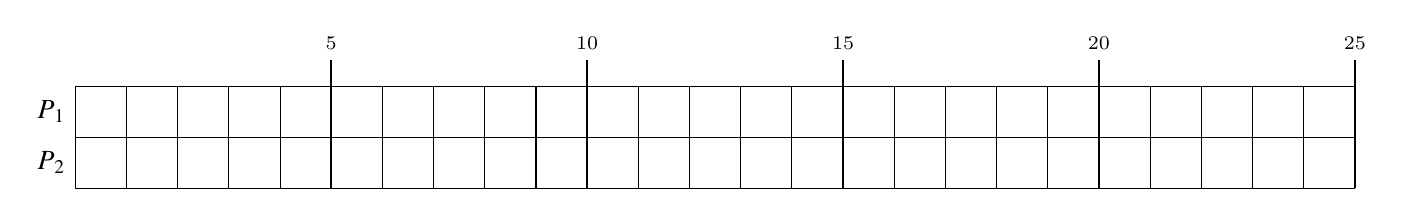
\begin{tikzpicture}[scale = 1.3, lbl/.style={font=\tiny, inner sep = 1 pt, fill = white}]
\path (0, 3/4) node[left] {$P_{1}$};
\path (0, 1/4) node[left] {$P_{2}$};
\draw[step=1/2] (0,0) grid (25/2, 2/2);
\foreach \i in {5, 10, ..., 25}{\draw[thick] (\i/2,0) -- (\i/2,2/2+1/4) node[font = \scriptsize, above]{\i};}
\end{tikzpicture} 
\end{center}

%\vfill

\item How much \emph{idle time} is in this schedule?%, and when?
 \hrulefill

\item How long did this schedule take to complete? \ans

\item %What is the critical path and the critical time for this digraph?

%\bigskip

Find the \emph{critical path} \hrulefill \emph{critical time} \ans

\item Is the schedule you found above optimal? Explain your answer: how do you know?

 % {\bf Scrub this part and divert points away from this problem?}

\vfill
\end{subproblems}

\newpage



% page 6 %

%%%%
%% priority lists, backflow
%%%%
%\problem{10 points} Consider the following digraph:
%\vspace*{-.3in}
%\begin{center}
%\anotherdigraph
%\end{center}
%
%\begin{subproblems}
%
%\item Construct the priority list for the digraph corresponding to the \emph{ decreasing time algorithm. } \\ 
%
%\hrulefill
%
%\item Label the vertices of the digraph according to the \emph{backflow algorithm.}
%
%\item Construct the {priority list} for the digraph corresponding to the \emph{critical path algorithm}. \\
%
%\hrulefill
%		
%\end{subproblems}

%%%
%Eulerization
%%%


%Page 7%

%%%%
% Dijkstra's Algorithm
%%%%
\problem{12 points} 

Recall Dijkstra's algorithm says the following: 

\bigskip
	
	\fbox{Dijkstra's Algorithm}

\emph{input:} a graph with distances (weights) on the edges and a starting vertex, say $s$\\
\emph{output:} the shortest distance between $s$ and every vertex in the graph\\
\emph{rough strategy:} All vertices get \emph{tentative} distances to vertex $s$. One-by-one, vertices are explored and tentative distances are updated until minimum distances are obtained. Break ties alphabetically.\\
	
	\begin{subproblems}
	
\item Use Dijkstra's algorithm to determine the distances between vertex $S$ and each other vertex. Clearly show the steps of the algorithm in the space provided.
	
	\def\ss{6}
\begin{center}
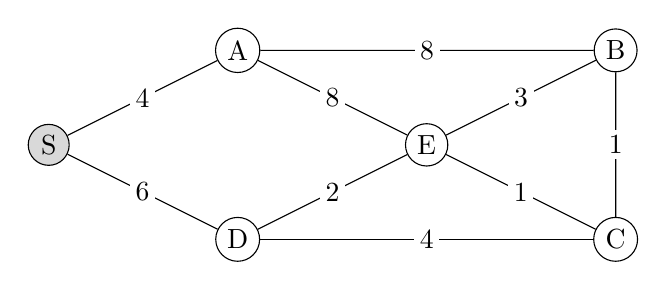
\begin{tikzpicture}[baseline=(current bounding box.center),lbl/.style={inner sep = 2pt, fill = white}, scale = 1.2]
\tikzstyle{vtx}=[circle, draw, inner sep=2pt]
\node[vtx, fill = gray!30] (s) at (0,1) {S};
\node[vtx] (a) at (2,2) {A};
\node[vtx] (d) at (2,0) {D};
\node[vtx] (e) at (4,1){E};
\node[vtx] (b) at (6,2){B};
\node[vtx] (c) at (6,0){C};
\foreach \i/\j/\k in {s/a/4,s/d/6,a/b/8,a/e/8,b/c/1,c/d/4,c/e/1,d/e/2, e/b/3}{\draw (\i) --node[lbl]{\k} (\j);}
\end{tikzpicture}
\end{center}

\begin{minipage}[t]{.6\linewidth}
\vspace{0pt}
\begin{tabular}{ c | c | p{1.5in}}
Explored? & vertices & tentative distances\\ \hline
&S& \\[12pt] \hline
&A& \\[12pt]\hline
&B& \\[12pt]\hline
&C& \\[12pt]\hline
&D& \\[12pt]\hline
&E& \\[12pt]\hline
 \end{tabular}

 \end{minipage}
% 
%\vspace{1cm}
%
 %
 \begin{minipage}[t]{.4\linewidth}
 \vspace{0pt}
   List the vertices in the order you \\ explored them. \\
   \underline{\hspace{5.5cm}}
     \vspace{1cm}
     
     List the \emph{final} distances to $S$.
     
     \bigskip

\begin{tabular}{c || c | c | c | c | c | c}
vertex & S & A &  B& C & D & E \\ \hline
distance from $S$ & &&&&& \\[12 pt]
\end{tabular}


 \end{minipage}

 \vspace{1cm}
 	
\item Which vertex is farthest away from S? \ans\  How far is it? \ans
\vfill

\end{subproblems}

\newpage
%
%\problem{12 points} VERSION 2
%Recall Dijkstra's algorithm says the following:
%	
%	\fbox{Dijkstra's Algorithm}
%
%\emph{input:} a graph with distances (weights) on the edges and a starting vertex, say $s$\\
%\emph{output:} the shortest distance between $s$ and every vertex in the graph\\
%\emph{rough strategy:} All vertices get \emph{tentative} distances to vertex $s$. One-by-one, vertices are explored and tentative distances are updated until minimum distances are obtained. Break ties alphabetically.\\
%	
%\begin{subproblems}
%	
%\item Use \emph{Dijkstra's algorithm} to determine the distances between vertex $S$
%and each other vertex. Clearly show the steps of the algorithm in the
%space provided.
%	
%	\begin{center}
%\begin{tikzpicture}[baseline=(current bounding box.center),lbl/.style={inner sep = 2pt, fill = white}, scale = 1.5]
%\tikzstyle{vtx}=[circle, draw, inner sep=2pt]
%\node[vtx, fill = gray!30] (S) at (90:2) {S};
%\node[vtx] (A) at (135:2) {A};
%\node[vtx] (C) at (90:0.5){C};
%\node[vtx] (E) at (-15:1.5){E};
%\node[vtx] (B) at (45:2) {B};
%\node[vtx] (D) at (15+180:1.5){D};
%\foreach \i/\j/\k in {S/A/5,S/B/3,A/C/4, A/D/2,B/C/7,B/E/12,C/E/6,C/D/1,D/E/3}{\draw (\i) --node[lbl]{\k} (\j);}
%\end{tikzpicture}
%\end{center}
%
%
%\begin{minipage}[t]{.6\linewidth}
%\vspace{0pt}
%\begin{tabular}{ c | c | p{1.5in}}
%Explored? & vertices & tentative distances\\ \hline
%&S& \\[12pt] \hline
%&A& \\[12pt]\hline
%&B& \\[12pt]\hline
%&C& \\[12pt]\hline
%&D& \\[12pt]\hline
%&E& \\[12pt]\hline
% \end{tabular}
%
% \end{minipage}
%% 
%%\vspace{1cm}
%%
% %
% \begin{minipage}[t]{.4\linewidth}
% \vspace{0pt}
%   List the vertices in the order you \\ explored them. \\
%   \underline{\hspace{5.5cm}}
%     \vspace{1cm}
%     
%     List the \emph{final} distances to $S$.
%     
%     \bigskip
%
%\begin{tabular}{c || c | c | c | c | c | c}
%vertex & $S$ & A &  B& C & D & E \\ \hline
%distance from $S$ & &&&&& \\[12 pt]
%\end{tabular}
%
%
% \end{minipage}
% 
% 
% \vspace{1cm}
% 	
%\item Which vertex is farthest away from $S$? \ans\  How far is it? \ans
%
%\end{subproblems}
%
%
%
%\newpage
% page 8 %

%%%%
%Extra Credit %
%\problem{} 
\emph{Extra Credit: (6 points)}

Consider the following digraph:
\begin{center}

\begin{tikzpicture}[vtx/.style={draw, circle, inner sep = 3pt, %font = \scriptsize
}, myto/.style={-latex, shorten >=2pt, shorten <=2pt
}, node distance = \r cm]
\node[vtx, label=above:{$A(3)$}, ] (A) at (0,0){};
\node[vtx, right = 2*\r of A, label=above:{ $B(5)$}] (B) {};
\node[vtx, below = of A, label=above:{ $C(7)$}] (C) {};
\node[vtx, right = 2*\r of C, label=above:{ $D(4)$}] (D) {};
\node[vtx, right = 2*\r of D, label=above:{ $E(1)$}] (E) {};
\node[vtx, below = of D, label=above:{ $F(6)$}] (F) {};
\foreach \i/\j in {A/B,C/D,C/F,D/E,B/E,F/E}{\draw[myto] (\i) -- (\j);}
% \draw[myto] (A) to[bend left = 20] (D);

\end{tikzpicture}

\end{center}

\begin{subproblems}

\item Construct the priority list for the digraph corresponding to the \emph{ decreasing time algorithm. } \\ 

\hrulefill

\item Label the vertices of the digraph according to the \emph{backflow algorithm.}

\item Construct the {priority list} for the digraph corresponding to the \emph{critical path algorithm}. \\

\hrulefill
		
\end{subproblems}





\end{document}

%%%%ENDDOCUMENT


